%======================
%   P3M コードの解説
%======================
\subsection{$\mathrm{P^{3}M}$コード} \label{subsec:P3M}
本節では、FDPSの拡張機能 Particle Mesh (以下、PMと省略する)の使用方法について、$\mathrm{P^{3}M}$(Particle-Particle-Particle-Mesh)法のサンプルコードを用いて解説を行う。このサンプルコードでは、塩化ナトリウム(NaCl)結晶の系全体の結晶エネルギーを$\mathrm{P^{3}M}$法で計算し、結果を解析解と比較する。$\mathrm{P^{3}M}$法では、力、及び、ポテンシャルエネルギーの計算を、Particle-Particle(PP)パートとParticle-Mesh(PM)パートにsplitして行われる。このサンプルコードではPPパートをFDPS標準機能を用いて計算し、PMパートをFDPS拡張機能を用いて計算する。なお、拡張機能PMの仕様の詳細は、仕様書9.2節で説明されているので、そちらも参照されたい。

\subsubsection{サンプルコードの場所と作業ディレクトリ}
サンプルコードの場所は、\dirNamePPPMSample である。まずは、そこに移動する。
\ifCpp % C++用
\begin{screen}
\begin{verbatim}
$ cd (FDPS)/sample/c++/p3m
\end{verbatim}
\end{screen}
サンプルコードは\texttt{main.cpp}とGCC用のMakefileである\texttt{Makefile}からなる。
\endifCpp
\ifFtn % Fortran用
\begin{screen}
\begin{verbatim}
$ cd (FDPS)/sample/fortran/p3m
\end{verbatim}
\end{screen}
サンプルコードはユーザ定義型と相互作用関数が実装された\texttt{user\_defined.F90}、ユーザコードのそれ以外の部分が実装された\texttt{f\_main.F90}、GCCとintelコンパイラ用のMakefileである\texttt{Makefile}と\texttt{Makefile.intel}から構成される。
\endifFtn
\ifC % C用
\begin{screen}
\begin{verbatim}
$ cd (FDPS)/sample/c/p3m
\end{verbatim}
\end{screen}
サンプルコードはユーザ定義型が実装された\texttt{user\_defined.h}、相互作用関数が実装された\texttt{user\_defined.c}、ユーザコードのそれ以外の部分が実装された\texttt{c\_main.c}、及び、GCC用のMakefileである\texttt{Makefile}から構成される。
\endifC

%#################
%   ユーザ定義型
%#################
\subsubsection{ユーザー定義型}
本節では、FDPSの機能を用いて$\mathrm{P^{3}M}$法の計算を行うにあたって、ユーザーが記述しなければならない\structure について記述する。

%---------------------
%   FullParticle型
%---------------------
\subsubsubsection{FullParticle型}
ユーザーはFullParticle型を記述しなければならない。Listing \ref{p3m_FP}に、サンプルコードのFullParticle型を示す。FullParticle型には、計算を行うにあたって、粒子が持っているべき全ての物理量が含まれている必要がある。
\ifCpp % C++用
また、以下のメンバ関数を持たせる必要がある:
\begin{itemize}[leftmargin=*,itemsep=-1ex]
\item \texttt{getCharge()} --- FDPSが粒子の電荷量を取得するのに必要
\item \texttt{getChargeParticleMesh()} --- FDPSのPMモジュールが粒子の電荷量を取得するために必要
\item \texttt{getPos()} --- FDPSが粒子座標を取得するのに必要
\item \texttt{getRSearch()} --- FDPSがカットオフ半径を取得するのに必要
\item \texttt{setPos()} --- FDPSが粒子の座標を書き込むのに必要
\item \texttt{copyFromForce()} --- Force型から結果をコピーするのに必要なメンバ関数
\item \texttt{copyFromForceParticleMesh()} --- PMモジュールが力の計算結果を書き込むために必要
\end{itemize}
なお、このサンプルコードでは\texttt{copyFromForce()}と\texttt{copyFromForceParticleMesh()}が空関数になっている。これはサンプルコードでは後述するAPI \texttt{getForce()}等を用いて、明示的に結果をForce型からFullParticle型にコピーする実装になっているためである。
\endifCpp

\ifCpp % C++用
\lstinputlisting[linerange={90-118},caption=FullParticle型,label=p3m_FP]{../../../../sample/c++/p3m/main.cpp}
\endifCpp
\ifFtn % Fortran用
\lstinputlisting[linerange={18-30},caption=FullParticle型,label=p3m_FP]{../../../../sample/fortran/p3m/user_defined.F90}
\endifFtn
\ifC % C用
\lstinputlisting[linerange={21-32},caption=FullParticle型,label=p3m_FP]{../../../../sample/c/p3m/user_defined.h}
\endifC

\ifIF % Fortran, C用
この \structure がFullParticle型であることを示すため、次の指示文を記述している:
\endifIF
\ifFtn % Fortran用
\begin{screen}
\begin{verbatim}
type, public, bind(c) :: nbody_fp !$fdps FP
\end{verbatim}
\end{screen}
\endifFtn
\ifC % C用
\begin{screen}
\begin{verbatim}
typedef struct fp_nbody { //$fdps FP
\end{verbatim}
\end{screen}
\endifC
\ifIF % Fortran,C用
$\mathrm{P^{3}M}$シミュレーションにおける相互作用はカットオフを持つ長距離力である。そのため、必須物理量としてカットオフ半径が加わる。現在のFDPSの仕様では、カットオフ半径の指定は探索半径の指定(\S~\ref{subsec:how_to_use:sph}参照)と同様に行う。次の指示文は、どのメンバ変数がどの必須物理量に対応するかを指定するものである:
\endifIF
\ifFtn % Fortran用
\begin{screen}
\begin{verbatim}
real(kind=c_double) :: m !$fdps charge
real(kind=c_double) :: rc !$fdps rsearch
type(fdps_f64vec) :: x !$fdps position
\end{verbatim}
\end{screen}
\endifFtn
\ifC % C用
\begin{screen}
\begin{verbatim}
double mass; //$fdps charge
double rcut; //$fdps rsearch     
fdps_f64vec pos; //$fdps position
\end{verbatim}
\end{screen}
\endifC
\ifIF % Fortran,C用
FullParticle型はForce型との間でデータコピーを行う。ユーザは指示文を使い、FDPSにデータコピーの仕方を教えなければならない。また、拡張機能PMを用いて相互作用計算を行う場合、FullParticle型にはPMモジュールで計算した相互作用計算の結果をどのメンバ変数で受け取るのか指示する指示文を記述する必要がある。本サンプルコードでは、以下のように記述している:
\endifIF
\ifFtn % Fortran用
\begin{screen}
\begin{verbatim}
!$fdps copyFromForce nbody_pp_results (pot,pot) (agrv,agrv)
!$fdps copyFromForcePM agrv_pm
\end{verbatim}
\end{screen}
\endifFtn
\ifC % C用
\begin{screen}
\begin{verbatim}
//$fdps copyFromForce force_pp (pot,pot) (acc,acc)  
//$fdps copyFromForcePM acc_pm                      
\end{verbatim}
\end{screen}
\endifC

%--------------------------
%   EssentialParticleI型
%--------------------------
\subsubsubsection{EssentialParticleI型}
ユーザーはEssentialParticleI型を記述しなければならない。EssentialParticleI型には、PPパートのForce計算を行う際、$i$粒子が持っているべき全ての物理量をメンバ変数として持っている必要がある。また、本チュートリアル中では、EssentialParticleJ型も兼ねているため、$j$粒子が持っているべき全ての物理量もメンバ変数として持っている必要がある。Listing \ref{p3m_EP}に、サンプルコードのEssentialParticleI型を示す。

\ifCpp % C++用
このEssentialParticleI型には前述したFullParticle型から、値をコピーするのに必要なメンバ関数\texttt{copyFromFP()}を持つ必要がある。その他、粒子の電荷量を返す関数である\texttt{getCharge()}、粒子座標を返す関数である\texttt{getPos()}、粒子のカットオフ半径を返す関数である\texttt{getRSearch()}、粒子の座標を書き込む関数である\texttt{setPos()}が必要になる。
\endifCpp

\ifCpp % C++用
\lstinputlisting[linerange={121-147},caption=EssentialParticleI型,label=p3m_EP]{../../../../sample/c++/p3m/main.cpp}
\endifCpp
\ifFtn % Fortran用
\lstinputlisting[linerange={33-39},caption=EssentialParticleI型,label=p3m_EP]{../../../../sample/fortran/p3m/user_defined.F90}
\endifFtn
\ifC % C用
\lstinputlisting[linerange={35-41},caption=EssentialParticleI型,label=p3m_EP]{../../../../sample/c/p3m/user_defined.h}
\endifC

\ifIF % Fortran,C用
まず、ユーザは指示文を用いて、この\structure がEssentialParticleI型かつEssentialParticleJ型であることをFDPSに教えなければならない。本サンプルコードでは、以下のように記述している:
\endifIF
\ifFtn % Fortran用
\begin{screen}
\begin{verbatim}
type, public, bind(c) :: nbody_ep !$fdps EPI,EPJ
\end{verbatim}
\end{screen}
\endifFtn
\ifC % C用
\begin{screen}
\begin{verbatim}
typedef struct ep_nbody { //$fdps EPI,EPJ
\end{verbatim}
\end{screen}
\endifC
\ifIF % Fortran,C用
次に、ユーザはこの\structure のどのメンバ変数がどの必須物理量に対応するのかを指示文によって指定しなければならない。今回は相互作用がカットオフ有りの長距離力であるため、カットオフ半径の指定も必要である。本サンプルコードでは、以下のように記述している:
\endifIF
\ifFtn % Fortran用
\begin{screen}
\begin{verbatim}
real(kind=c_double) :: m !$fdps charge
real(kind=c_double) :: rc !$fdps rsearch
type(fdps_f64vec) :: x !$fdps position
\end{verbatim}
\end{screen}
\endifFtn
\ifC % C用
\begin{screen}
\begin{verbatim}
double mass; //$fdps charge         
double rcut; //$fdps rsearch        
fdps_f64vec pos; //$fdps position   
\end{verbatim}
\end{screen}
\endifC
\ifIF % Fortran,C用
EssentialParticleI 型と EssentialParticleJ 型は FullParticle 型からデータを受け取る。ユーザは FullParticle 型のどのメンバ変数を EssentialParticle?型 (?=I,J) のどのメンバ変数にコピーするのかを、指示文を用いて指定する必要がある。本サンプルコードでは、以下のように記述している:
\endifIF
\ifFtn % Fortran用
\begin{screen}
\begin{verbatim}
!$fdps copyFromFP nbody_fp (id,id) (m,m) (rc,rc) (x,x)
\end{verbatim}
\end{screen}
\endifFtn
\ifC % C用
\begin{screen}
\begin{verbatim}
//$fdps copyFromFP fp_nbody (id,id) (mass,mass) (rcut,rcut) (pos,pos)
\end{verbatim}
\end{screen}
\endifC

%-------------
%   Force型
%-------------
\subsubsubsection{Force型}
ユーザーはForce型を記述しなければならない。Force型は、PPパートのForceの計算を行った際にその結果として得られる全ての物理量をメンバ変数として持っている必要がある。本サンプルコードのForce型をListing \ref{p3m_force}に示す。このサンプルコードでは、ForceはCoulomb相互作用計算のみであるため、Force型が1つ用意されている。
\ifCpp % C++用
また、積算対象のメンバ変数を0ないし初期値に設定するための関数\texttt{clear()}が必要になる。
\endifCpp

\ifCpp % C++用
\lstinputlisting[linerange={78-87},caption=Force型,label=p3m_force]{../../../../sample/c++/p3m/main.cpp}
\endifCpp
\ifFtn % Fortran用
\lstinputlisting[linerange={11-15},caption=Force型,label=p3m_force]{../../../../sample/fortran/p3m/user_defined.F90}
\endifFtn
\ifC % C用
\lstinputlisting[linerange={14-18},caption=Force型,label=p3m_force]{../../../../sample/c/p3m/user_defined.h}
\endifC

\ifIF % Fortran,C用
まず、ユーザはこの\structure がForce型であることを指示文によって指定する必要がある。本サンプルコードでは、以下のように記述している:
\endifIF
\ifFtn % Fortran用
\begin{screen}
\begin{verbatim}
type, public, bind(c) :: nbody_pp_results !$fdps Force
\end{verbatim}
\end{screen}
\endifFtn
\ifC % C用
\begin{screen}
\begin{verbatim}
typedef struct force_pp { //$fdps Force
\end{verbatim}
\end{screen}
\endifC
\ifIF % Fortran,C用
この\structure はForce型であるから、ユーザは\ulBold{必ず}、相互作用計算における積算対象のメンバ変数の初期化方法を指定する必要がある。本サンプルコードではForce型のすべてのメンバ変数にデフォルトの初期化方法を指定するため、単に、キーワード\texttt{clear}の指示文を記述している:
\endifIF
\ifFtn % Fortran
\begin{screen}
\begin{verbatim}
!$fdps clear
\end{verbatim}
\end{screen}
\endifFtn
\ifC % C用
\begin{screen}
\begin{verbatim}
//$fdps clear
\end{verbatim}
\end{screen}
\endifC

%---------------------
%   calcForceEpEp
%---------------------
\subsubsubsection{相互作用関数 calcForceEpEp} \label{subsubsubsec:p3m_calcForceEpEp}
ユーザーは相互作用関数 calcForceEpEpを記述しなければならない。calcForceEpEpには、PPパートのForceの計算の具体的な内容を書く必要がある。calcForceEpEp は、\procedure \describeForCpp{或いは、ファンクタ(関数オブジェクト)}として実装されなければならない。引数は、EssentialParticleIの配列、EssentialParticleIの個数、EssentialParticleJの配列、EssentialParticleJの個数、Force型の配列である。本サンプルコードのcalcForceEpEpの実装をListing \ref{p3m_calcForceEpEp}に示す。\describeForCpp{このサンプルコードでは、ファンクタ(関数オブジェクト)を用いて実装している。}

\ifCpp % C++用
\lstinputlisting[linerange={150-174},caption=相互作用関数 calcForceEpEp,label=p3m_calcForceEpEp]{../../../../sample/c++/p3m/main.cpp}
\endifCpp
\ifFtn % Fortran用
\lstinputlisting[linerange={121-152},caption=相互作用関数 calcForceEpEp,label=p3m_calcForceEpEp]{../../../../sample/fortran/p3m/user_defined.F90}
\endifFtn
\ifC % C用
\lstinputlisting[linerange={58-85},caption=相互作用関数 calcForceEpEp,label=p3m_calcForceEpEp]{../../../../sample/c/p3m/user_defined.c}
\endifC

% カットオフ関数
$\mathrm{P^{3}M}$法のPPパートは、(距離に関する)カットオフ付きの2体相互作用である。そのため、ポテンシャルと加速度の計算にカットオフ関数(\texttt{S2\_pcut()}, \texttt{S2\_fcut()})が含まれていることに注意されたい。ここで、各カットオフ関数は、粒子の形状関数$S(r)$が$S2(r)$のときのカットオフ関数である必要がある。ここで、$S2(r)$はHockney \& Eastwood (1988)の式(8.3)で定義される形状関数で、以下の形を持つ:
\begin{equation}
S2(r) = \left\{
\begin{array}{ll}
\dfrac{48}{\pi a^{4}}\left(\dfrac{a}{2}-r\right) & r < a/2, \\
0 & \mathrm{otherwise}.
\end{array}
\right.
\end{equation}
ここで、$r$は粒子からの距離、$a$は形状関数のスケール長である。粒子の電荷量を$q$とすれば、この粒子が作る電荷密度分布$\rho(r)$は$\rho(r)=q\,S2(r)$と表現される。これは$r$に関して線形な密度分布を仮定していることを意味する。PPパートのカットオフ関数が$S2(r)$を仮定したものでなければならない理由は、PMパートのカットオフ関数がS2型形状関数を仮定して実装されているためである(PMパートとPPパートのカットオフ関数は同じ形状関数に基づく必要がある)。

% カットオフ関数の実装例
カットオフ関数はユーザが定義する必要がある。サンプルコードの冒頭に\texttt{S2\_pcut()}と\texttt{S2\_fcut()}の実装例がある。これらの関数では、Hockney \& Eastwood (1988)の式(8-72),(8-75)が使用されている。カットオフ関数は、PP相互作用が以下の形となるように定義されている:
\begin{eqnarray}
\Phi_{\mathrm{PP}}(\bm{r}) & = & \dfrac{m}{|\bm{r}-\bm{r}'|}\mathtt{S2\_pcut}(\xi) \\
\bm{f}_{\mathrm{PP}}(\bm{r}) & = & \dfrac{m(\bm{r}-\bm{r}')}{|\bm{r}-\bm{r}'|^{3}}\mathtt{S2\_fcut}(\xi)
\end{eqnarray}
ここで、$\xi = 2|\bm{r}-\bm{r}'|/a$である。
本サンプルコードでは$a$を変数\describeForEach{\texttt{rc}}{\texttt{rc}}{\texttt{rcut}}で表現している。

% 自己相互作用項について
Hockney \& Eastwood (1988)の式(8-75)を見ると、$r=0$のとき、メッシュポテンシャル$\phi^{m}$が次の有限値を持つことがわかる(ここで、$1/4\pi\varepsilon_{0}$の因子は省略した):
\begin{equation}
\phi^{m}(0) = \dfrac{208}{70a}
\end{equation}
この項はサンプルコードの$i$粒子のループの最後で考慮されている:
\ifCpp
\begin{lstlisting}
result[i].pot -= ep_i[i].m * (208.0/(70.0*ep_i[i].rc));
\end{lstlisting}
\endifCpp
\ifFtn
\begin{lstlisting}
f(i)%pot = f(i)%pot - ep_i(i)%m * (208.0d0/(70.0d0*ep_i(i)%rc))
\end{lstlisting}
\endifFtn
\ifC
\begin{lstlisting}
f[i].pot -= ep_i[i].mass * (208.0/(70.0*ep_i[i].rcut));
\end{lstlisting}
\endifC

この項を考慮しないと解析解と一致しないことに注意する必要がある。

%---------------------
%   calcForceEpSp
%---------------------
\subsubsubsection{相互作用関数 calcForceEpSp} \label{subsubsubsec:p3m_calcForceEpSp}
ユーザーは相互作用関数 calcForceEpSpを記述しなければならない\footnote{冒頭で述べたように、本サンプルコードでは相互作用計算に$\mathrm{P^{3}M}$法を用いる。FDPSの枠組み内で、これを実現するため、後述するように、見込み角の基準値$\theta$を0に指定して相互作用計算を行う。このため、粒子-超粒子相互作用は発生しないはずである。しかしながら、API \describeForEach{\texttt{calcForceAllAndWriteBack}}{\texttt{calc\_force\_all\_and\_write\_back}}{\texttt{fdps\_calc\_force\_all\_and\_write\_back}}に、粒子-超粒子間相互作用を計算する関数のアドレスを渡す必要があるため、相互作用関数 calcForceEpSp を定義する必要がある。}。calcForceEpSpには、粒子-超粒子間相互作用計算の具体的な内容を書く必要がある。calcForceEpSp は、\procedure \describeForCpp{或いは、ファンクタ(関数オブジェクト)}として実装されなければならない。引数は、EssentialParticleIの配列、EssentialParticleIの個数、超粒子型の配列、超粒子型の個数、Force型の配列である。本サンプルコードのcalcForceEpSpの実装をListing \ref{p3m_calcForceEpSp}に示す。\describeForCpp{このサンプルコードでは、ファンクタ(関数オブジェクト)を用いて実装している。}

\ifCpp % C++用
\lstinputlisting[linerange={175-195},caption=相互作用関数 calcForceEpSp,label=p3m_calcForceEpSp]{../../../../sample/c++/p3m/main.cpp}
\endifCpp
\ifFtn % Fortran用
\lstinputlisting[linerange={155-183},caption=相互作用関数 calcForceEpSp,label=p3m_calcForceEpSp]{../../../../sample/fortran/p3m/user_defined.F90}
\endifFtn
\ifC % C用
\lstinputlisting[linerange={87-111},caption=相互作用関数 calcForceEpSp,label=p3m_calcForceEpSp]{../../../../sample/c/p3m/user_defined.c}
\endifC


%-------------------
%   プログラム本体
%-------------------
\subsubsection{プログラム本体}
本節では、サンプルコード本体について解説を行う。詳細な説明に入る前に、サンプルコードの内容と全体構造について説明を与える。\ref{subsec:P3M}節で述べたように、このサンプルコードではNaCl結晶の結晶エネルギーを$\mathrm{P^{3}M}$法によって計算し解析解と比較する。NaCl結晶は一様格子状に並んだ粒子として表現される。NaとClは互い違いに並んでおり、Naに対応する粒子は正の電荷を、Clに対応する粒子は負の電荷を持っている。この粒子で表現された結晶を、大きさが$[0,1)^{3}$の周期境界ボックスの中に配置し、結晶エネルギーを計算する。結晶エネルギーの計算精度は周期境界ボックスの中の粒子数や粒子の配置に依存するはずなので、サンプルコードでは、これらを変えてエネルギーの相対誤差を調べ、結果をファイルに出力する内容となっている。

コードの全体構造は以下のようになっている:
\begin{enumerate}[leftmargin=*,itemsep=-1ex,label={(\arabic*)}]
\item FDPSで使用するオブジェクトの生成と初期化
\item 指定された粒子数と配置の結晶を生成 (\mainFunc の\describeForEach{\texttt{NaCl\_IC()}}{\texttt{setup\_NaCl\_crystal()}}{\texttt{setup\_NaCl\_crystal()}})
\item 各粒子のポテンシャルエネルギーを$\mathrm{P^{3}M}$法で計算 (\describeForEach{\mainFunc の\texttt{Nbody\_objs.calc\_gravity()}}{\mainFunc 内}{\mainFunc 内})
\item 系全体のエネルギーを計算し、解析解と比較 (\mainFunc の\texttt{calc\_energy\_error()})
\item (2)〜(4)を繰り返す
\end{enumerate}

以下で、個々について詳しく説明を行う。

\ifCpp % C++用
\subsubsection{ヘッダファイルのインクルード}
拡張機能PMをFDPS標準機能とともに使用するため、\texttt{particle\_simulator.hpp}に加え、\texttt{particle\_mesh.hpp}と\texttt{param\_fdps.h}をインクルードする。これに加え、このサンプルコードでは拡張機能の非公開定数\texttt{CUTOFF\_RADIUS}を参照するため、\texttt{param.h}もインクルードしている。
\begin{lstlisting}[caption=Include FDPS]
#include <particle_simulator.hpp>
#include <particle_mesh.hpp>
#include <param.h>
#include <param_fdps.h>
\end{lstlisting}
\endifCpp
\ifFtn % Fortran用
\subsubsubsection{\texttt{fdps\_controller}型オブジェクトの生成}
FDPS Fortran インターフェースにおいて、FDPSのAPIはすべてFortran 2003のクラス\texttt{FDPS\_controller}のメンバ関数として提供される。このクラスは、インターフェースプログラムの1つである\texttt{FDPS\_module.F90}の中の、モジュール\texttt{fdps\_module}内で定義されている。したがって、ユーザはFDPSのAPIを使用するために、\texttt{FDPS\_controller}型オブジェクトを生成しなければならない。本サンプルコードでは、\texttt{FDPS\_controller}型オブジェクト\texttt{fdps\_ctrl}をメインルーチンで生成している:
\begin{lstlisting}[caption=\texttt{fdps\_controller}型オブジェクトの生成]
subroutine f_main()
   use fdps_module
   implicit none
   !* Local variables
   type(fdps_controller) :: fdps_ctrl
    
   ! Do something
   
end subroutine f_main    
\end{lstlisting}
ここに示したコードは実際にサンプルコードから必要な部分だけを取り出したものであることに注意して頂きたい。

上記の理由から、以下の説明において、FDPSのAPIはこのオブジェクトのメンバ関数として呼び出されていることに注意されたい。
\endifFtn
\ifC % C用
\subsubsubsection{ヘッダーファイルのインクルード}
FDPSの標準機能を利用できるようにするため、\texttt{FDPS\_c\_if.h}をインクルードする。
\begin{lstlisting}[caption=ヘッダーファイル\texttt{FDPS\_c\_if.h}のインクルード]
#include "FDPS_c_if.h"
\end{lstlisting}
\endifC


\subsubsubsection{開始、終了}
まずは、FDPSの初期化/開始を行う必要がある。
次のように、\mainFunc に記述する。

\ifCpp % C++用
\begin{lstlisting}[caption=FDPSの開始]
PS::Initialize(argc, argv);
\end{lstlisting}
\endifCpp
\ifFtn % Fortran用
\begin{lstlisting}[caption=FDPSの開始]
fdps_ctrl%ps_initialize();
\end{lstlisting}
\endifFtn
\ifC % C用
\begin{lstlisting}[caption=FDPSの開始]
fdps_initialize();
\end{lstlisting}
\endifC


FDPSは、開始したら明示的に終了させる必要がある。今回は、プログラムの終了と同時にFDPSも終了させるため、\mainFunc の最後に次のように記述する。

\ifCpp % C++用
\begin{lstlisting}[caption=FDPSの終了]
PS::Finalize();
\end{lstlisting}
\endifCpp
\ifFtn % Fortran用
\begin{lstlisting}[caption=FDPSの終了]
fdps_ctrl%ps_finalize();
\end{lstlisting}
\endifFtn
\ifC % C用
\begin{lstlisting}[caption=FDPSの終了]
fdps_finalize();
\end{lstlisting}
\endifC

\subsubsubsection{オブジェクトの生成と初期化}
FDPSの初期化に成功した場合、ユーザーはコード中で用いるオブジェクトを作成する必要がある。
本節では、オブジェクトの生成/初期化の仕方について、解説する。

\subsubsubsubsection{オブジェクトの生成}
$\mathrm{P^{3}M}$法の計算では、粒子群クラス、領域クラスに加え、PPパートの計算用のtreeを1本、さらにPMパートの計算に必要なParticleMeshオブジェクトの生成が必要である。

\ifCpp % C++用
サンプルコードでは、これらのオブジェクトを\texttt{Nbody\_Objects}クラスにまとめている。以下にそのコードを記す。
\begin{lstlisting}[caption=\texttt{Nbody\_Objects}クラス]
class Nbody_Objects {
   public:
      PS::ParticleSystem<Nbody_FP> system;
      PS::DomainInfo dinfo;
      PS::TreeForForceLong<Nbody_PP_Results, Nbody_EP, Nbody_EP>::MonopoleWithCutoff pp_tree;
      PS::PM::ParticleMesh pm;
}
\end{lstlisting}
サンプルコードでは、メイン関数のローカル変数として\texttt{Nbody\_Objects}オブジェクトを1個生成している:
\begin{lstlisting}[caption=\texttt{Nbody\_Objects}クラスのオブジェクト生成]
Nbody_Objects Nbody_objs;
\end{lstlisting}
\endifCpp

\ifFtn % Fortran用
\begin{lstlisting}[caption=オブジェクトの生成]
call fdps_ctrl%create_psys(psys_num,'nbody_fp')
call fdps_ctrl%create_dinfo(dinfo_num)
call fdps_ctrl%create_pm(pm_num)
call fdps_ctrl%create_tree(tree_num, &                                                  
                           "Long,nbody_pp_results,nbody_ep,nbody_ep,MonopoleWithCutoff")
\end{lstlisting}
ここに示したコードは実際にサンプルコードから該当箇所だけを取り出したものであることに注意して頂きたい。
\endifFtn
\ifC % C用
\begin{lstlisting}[caption=オブジェクトの生成]
fdps_create_psys(&psys_num,"fp_nbody");
fdps_create_dinfo(&dinfo_num);
fdps_create_pm(&pm_num);
fdps_create_tree(&tree_num,
                 "Long,force_pp,ep_nbody,ep_nbody,MonopoleWithCutoff");
\end{lstlisting}
ここに示したコードは実際にサンプルコードから該当箇所だけを取り出したものであることに注意して頂きたい。
\endifC

\subsubsubsubsection{オブジェクトの初期化}
ユーザーはオブジェクトを生成したら、そのオブジェクトを使用する前に、初期化を行う必要がある。以下で、各オブジェクトの初期化の仕方について解説を行う。

\begin{description}[leftmargin=*]
\item[(i) 粒子群オブジェクトの初期化]
粒子群オブジェクトの初期化は、以下のように行う:
\ifCpp % C++用
\begin{lstlisting}[caption=粒子群オブジェクトの初期化]
Nbody_objs.system.initialize();
\end{lstlisting}
\endifCpp
\ifFtn % Fortran用
\begin{lstlisting}[caption=粒子群オブジェクトの初期化]
call fdps_ctrl%init_psys(psys_num)
\end{lstlisting}
\endifFtn
\ifC % C用
\begin{lstlisting}[caption=粒子群オブジェクトの初期化]
fdps_init_psys(psys_num);
\end{lstlisting}
\endifC
サンプルコードでは\mainFunc の冒頭で呼び出されている。

\item[(ii) 領域オブジェクトの初期化]
領域オブジェクトの初期化は、以下のように行う:
\ifCpp % C++用
\begin{lstlisting}[caption=領域オブジェクトの初期化]
Nbody_objs.dinfo.initialize();
\end{lstlisting}
\endifCpp
\ifFtn % Fortran用
\begin{lstlisting}[caption=領域オブジェクトの初期化]
call fdps_ctrl%init_dinfo(dinfo_num,coef_ema)
\end{lstlisting}
\endifFtn
\ifC % C用
\begin{lstlisting}[caption=領域オブジェクトの初期化]
fdps_init_dinfo(dinfo_num,coef_ema);
\end{lstlisting}
\endifC
サンプルコードでは\mainFunc の冒頭で呼び出されている。

初期化が完了した後、領域オブジェクトには境界条件と境界の大きさをセットする必要がある。
サンプルコードでは、この作業は粒子分布を決定する\procedure \describeForEach{\texttt{NaCl\_IC()}}{\texttt{setup\_NaCl\_crystal}}{\texttt{setup\_NaCl\_crystal}}の中で行われている:
\ifCpp % C++用
\begin{lstlisting}
dinfo.setBoundaryCondition(PS::BOUNDARY_CONDITION_PERIODIC_XYZ);
dinfo.setPosRootDomain(PS::F64vec(0.0,0.0,0.0),
                       PS::F64vec(1.0,1.0,1.0));
\end{lstlisting}
\endifCpp
\ifFtn % Fortran用
\begin{lstlisting}
call fdps_ctrl%set_boundary_condition(dinfo_num,fdps_bc_periodic_xyz)
pos_ll%x = 0.0d0; pos_ll%y = 0.0d0; pos_ll%z = 0.0d0
pos_ul%x = 1.0d0; pos_ul%y = 1.0d0; pos_ul%z = 1.0d0
call fdps_ctrl%set_pos_root_domain(dinfo_num,pos_ll,pos_ul)
\end{lstlisting}
\endifFtn
\ifC % C用
\begin{lstlisting}
fdps_set_boundary_condition(dinfo_num,FDPS_BC_PERIODIC_XYZ);
fdps_f32vec pos_ll, pos_ul;
pos_ll.x = 0.0; pos_ll.y = 0.0; pos_ll.z = 0.0;
pos_ul.x = 1.0; pos_ul.y = 1.0; pos_ul.z = 1.0;
fdps_set_pos_root_domain(dinfo_num,&pos_ll,&pos_ul);
\end{lstlisting}
\endifC

\item[(iii) ツリーオブジェクトの初期化]
相互作用ツリーオブジェクトの初期化も、API \describeForEach{\texttt{initialize}}{\texttt{init\_tree}}{\texttt{fdps\_init\_tree}}を使って、以下のように行う:
\ifCpp
\begin{lstlisting}[caption=ツリーオブジェクトの初期化]
void init_tree() {
   PS::S32 numPtclLobal = system.getNumberOfParticleLobal();
   PS::U64 ntot = 3 * numPtclLobal;
   pp_tree.initialize(ntot,0.0);
}; 
\end{lstlisting}
\endifCpp
\ifFtn
\begin{lstlisting}[caption=ツリーオブジェクトの初期化]
call fdps_ctrl%init_tree(tree_num,3*nptcl_loc,theta, &
                         n_leaf_limit,n_group_limit)
\end{lstlisting}
\endifFtn
\ifC
\begin{lstlisting}[caption=ツリーオブジェクトの初期化]
fdps_init_tree(tree_num,3*nptcl_loc,theta,
               n_leaf_limit,n_group_limit);
\end{lstlisting}
\endifC
ツリーオブジェクトのAPI \describeForEach{\texttt{initialize}}{\texttt{init\_tree}}{\texttt{fdps\_init\_tree}}には引数として、大雑把な粒子数を渡す必要がある。これはAPIの第\describeForEach{1}{2}{2}引数として指定する。上記の例では、APIが呼ばれた時点でのローカル粒子数の3倍の値がセットされるようになっている。一方、APIの第\describeForEach{2}{3}{3}引数は\describeForEach{省略可能引数で}{省略可能引数で}{}、tree法で力を計算するときのopening angle criterion $\theta$を指定する。本サンプルコードではPPパートの計算で粒子-超粒子相互作用を発生させないようにするため、$\theta=0$を指定している。

\ifCpp
本サンプルコードでは、ツリーオブジェクトの初期化は\texttt{Nbody\_objs.init\_tree()}を通して行っている(メイン関数を参照のこと)。
\begin{lstlisting}
if (is_tree_initialized == false) {
   Nbody_objs.init_tree();
   is_tree_initialized = true;
}
\end{lstlisting}
ここで、初期化はプログラム中で1回だけ行う必要があるため、上記のようなif文の処理が必要となる。
\endifCpp


\item[(iv) ParticleMeshオブジェクトの初期化] 特に明示的に初期化を行う必要はない。

\end{description}

\subsubsubsection{粒子分布の生成}
本節では、粒子分布を生成する\procedure \describeForEach{\texttt{NaCl\_IC}}{\texttt{setup\_NaCl\_crystal}}{\texttt{setup\_NaCl\_crystal}}の動作とその中で呼ばれているFDPSのAPIについて解説を行う。この\procedure は、周期境界ボックスの1次元あたりの粒子数と、原点$(0,0,0)$に最も近い粒子の座標を引数として、3次元粒子分布を生成する。サンプルコードでは、これらのパラメータは\structure \describeForEach{\texttt{Crystal\_Parameters}}{\texttt{crystal\_parameters}}{\texttt{crystal\_parameters}}のオブジェクト\texttt{NaCl\_params}を使って渡されている:
\ifCpp
\begin{lstlisting}
class Crystal_Parameters
{
   public:
      PS::S32 numPtcl_per_side;
      PS::F64vec pos_vertex;
};
/* In main function */
Crystal_Parameters NaCl_params;
NaCl_IC(Nbody_objs.system,
        Nbody_objs.dinfo,
        NaCl_params);
\end{lstlisting}
\endifCpp
\ifFtn
\begin{lstlisting}
! In user_defined.F90
type, public, bind(c) :: crystal_parameters
   integer(kind=c_int) :: nptcl_per_side
   type(fdps_f64vec) :: pos_vertex
end type crystal_parameters
! In f_main.F90
type(crystal_parameters) :: NaCl_params
call setup_NaCl_crystal(fdps_ctrl, &
                        psys_num,  &
                        dinfo_num, &
                        NaCl_params)
\end{lstlisting}
\endifFtn
\ifC
\begin{lstlisting}
// In user_defined.h
typedef struct crystal_parameters {
   int nptcl_per_side;
   fdps_f64vec pos_vertex;
} Crystal_parameters;
// In c_main.c
Crystal_parameters NaCl_params;
setup_NaCl_crystal(psys_num, dinfo_num, NaCl_params);
\end{lstlisting}
\endifC

\describeForEach{\texttt{NaCl\_IC}}{\texttt{setup\_NaCl\_crystal}}{\texttt{setup\_NaCl\_crystal}}の前半部分において、渡されたパラメータを使って粒子分布を生成している。この結晶の系全体のエネルギーは
\begin{equation}
E = - \dfrac{N\alpha m^{2}}{R_{0}}
\end{equation}
と解析的に書ける。ここで、$N$は分子の総数(原子の数は$2N$個)、$m$は粒子の電荷量、$R_{0}$は最隣接原子間距離、$\alpha$はマーデリング(Madelung)定数である。NaCl結晶の場合、$\alpha\approx 1.747565$である(例えば、キッテル著 「固体物理学入門(第8版)」を参照せよ)。計算結果をこの解析解と比較するとき、系全体のエネルギーが粒子数に依存しては不便である。そこで、サンプルコードでは、系全体のエネルギーが粒子数に依存しないように、粒子の電荷量$m$を
\begin{equation}
\dfrac{2Nm^{2}}{R_{0}}=1
\end{equation}
となるようにスケールしていることに注意されたい。

粒子分布の生成後、FDPSのAPIを使って、領域分割と粒子交換を行っている。
以下で、これらのAPIについて解説する。

\subsubsubsubsection{領域分割の実行}
粒子分布に基いて領域分割を実行するには、領域オブジェクトのAPI \describeForEach{\texttt{decomposeDomainAll}}{\texttt{decompose\_domain\_all}}{\texttt{fdps\_decompose\_domain\_all}}を使用する:
\ifCpp
\begin{lstlisting}[caption=領域分割の実行]
dinfo.decomposeDomainAll(system);
\end{lstlisting}
ここで、粒子分布の情報を領域オブジェクトに与えるため、引数に粒子群オブジェクトが渡されていることに注意されたい。
\endifCpp
\ifFtn
\begin{lstlisting}[caption=領域分割の実行]
call fdps_ctrl%decompose_domain_all(dinfo_num,psys_num)
\end{lstlisting}
\endifFtn
\ifC
\begin{lstlisting}[caption=領域分割の実行]
fdps_decompose_domain_all(dinfo_num,psys_num);
\end{lstlisting}
\endifC


\subsubsubsubsection{粒子交換の実行}
領域情報に基いてプロセス間の粒子の情報を交換するには、粒子群オブジェクトのAPI \describeForEach{\texttt{exchangeParticle}}{\texttt{exchange\_particle}}{\texttt{fdps\_exchange\_particle}}を使用する:
\ifCpp
\begin{lstlisting}[caption=粒子交換の実行]
system.exchangeParticle(dinfo);
\end{lstlisting}
ここで領域情報を粒子群オブジェクトに与えるため、引数に領域オブジェクトが渡されていることに注意する。
\endifCpp
\ifFtn
\begin{lstlisting}[caption=粒子交換の実行]
call fdps_ctrl%exchange_particle(psys_num,dinfo_num)
\end{lstlisting}
\endifFtn
\ifC
\begin{lstlisting}[caption=粒子交換の実行]
fdps_exchange_particle(psys_num,dinfo_num);
\end{lstlisting}
\endifC

\subsubsubsection{相互作用計算の実行}
粒子分布を決定し、領域分割・粒子交換が終了したら、相互作用の計算を行う。
サンプルコードでは、この作業を\mainFunc で行っている:
\ifCpp
\begin{lstlisting}[caption=相互作用計算の実行]
Nbody_objs.calc_gravity();
\end{lstlisting}

\texttt{Nbody\_objs.calc\_gravity()}の中身は以下のようになっており、(i) ポテンシャルエネルギーと加速度の0クリア、(ii) PMパートの計算、(iii) PPパートの計算から構成される:
\begin{lstlisting}[caption=相互作用計算の中身]
void calc_gravity() {
   //* Local variables
   PS::S32 numPtclLocal = system.getNumberOfParticleLocal();

   //* Reset potential and accelerations
   for (PS::S32 i=0; i<numPtclLocal; i++) {
      system[i].pot  = 0.0;
      system[i].agrv = 0.0;
   }

   //=================
   //* [1] PM part 
   //=================
   pm.setDomainInfoParticleMesh(dinfo);
   pm.setParticleParticleMesh(system);
   pm.calcMeshForceOnly();
   for (PS::S32 i=0; i<numPtclLocal; i++) {
      PS::F32vec x32 = system[i].x;
      system[i].pot  -= pm.getPotential(x32);
      system[i].agrv -= pm.getForce(x32);
   }

   //=================                                                                   
   //* [2] PP part                                                                           
   //=================                                                                   
   pp_tree.calcForceAll(Calc_force_ep_ep(),                                              
                        Calc_force_ep_sp(),                                              
                        system, dinfo);                                                  
   for (PS::S32 i=0; i<numPtclLocal; i++) {                                              
      Nbody_PP_Results result = pp_tree.getForce(i);                                     
      system[i].pot  += result.pot;                                                      
      system[i].agrv += result.agrv;                                                     
   }
};
\end{lstlisting}
\endifCpp
\ifFtn
\begin{lstlisting}[caption=相互作用計算の実行]
!* [4] Compute force and potential with P^{3}M method
!* [4-1] Get the pointer to FP and # of local particles
nptcl_loc = fdps_ctrl%get_nptcl_loc(psys_num)
call fdps_ctrl%get_psys_fptr(psys_num,ptcl)
!* [4-2] PP part
pfunc_ep_ep = c_funloc(calc_force_ep_ep)
pfunc_ep_sp = c_funloc(calc_force_ep_sp)
call fdps_ctrl%calc_force_all_and_write_back(tree_num,    &
                                             pfunc_ep_ep, &
                                             pfunc_ep_sp, &
                                             psys_num,    &
                                             dinfo_num)
!* [4-3] PM part
call fdps_ctrl%calc_pm_force_all_and_write_back(pm_num,   &
                                                psys_num, &
                                                dinfo_num)
do i=1,nptcl_loc
   pos32 = ptcl(i)%x
   call fdps_ctrl%get_pm_potential(pm_num,pos32,ptcl(i)%pot_pm)
end do
!* [4-4] Compute the total acceleration and potential
do i=1,nptcl_loc
   ptcl(i)%pot  = ptcl(i)%pot  - ptcl(i)%pot_pm
   ptcl(i)%agrv = ptcl(i)%agrv - ptcl(i)%agrv_pm
end do
\end{lstlisting}
\endifFtn
\ifC
\begin{lstlisting}[caption=相互作用計算の実行]
// [4] Compute force and potential with P^{3}M method
// [4-1] Get the pointer to FP and # of local particles
int nptcl_loc = fdps_get_nptcl_loc(psys_num);
FP_nbody *ptcl = (FP_nbody *) fdps_get_psys_cptr(psys_num);
// [4-2] PP part
fdps_calc_force_all_and_write_back(tree_num,
                                   calc_force_ep_ep,
                                   calc_force_ep_sp,
                                   psys_num,
                                   dinfo_num,
                                   true,
                                   FDPS_MAKE_LIST);
// [4-3] PM part
fdps_calc_pm_force_all_and_write_back(pm_num,
                                      psys_num,
                                      dinfo_num);
int i;
for (i = 0; i < nptcl_loc; i++) {
   fdps_f32vec pos32;
   pos32.x = ptcl[i].pos.x;
   pos32.y = ptcl[i].pos.y;
   pos32.z = ptcl[i].pos.z;
   fdps_get_pm_potential(pm_num,&pos32,&ptcl[i].pot_pm);
}
// [4-4] Compute the total acceleration and potential
for (i = 0; i < nptcl_loc; i++) {
   ptcl[i].pot -= ptcl[i].pot_pm;
   ptcl[i].acc.x -= ptcl[i].acc_pm.x;
   ptcl[i].acc.y -= ptcl[i].acc_pm.y;
   ptcl[i].acc.z -= ptcl[i].acc_pm.z;
}
\end{lstlisting}
\endifC
\ifCpp
PMパートの計算部分を以下に示す。PMのForce計算を行うためには、ParticleMeshオブジェクト\texttt{pm}が領域情報と粒子情報を事前に知っている必要がある。そのため、サンプルコードでは、まず、API \texttt{setDomainInfoParticleMesh}と\texttt{setParticleParticleMesh}で、領域情報と粒子情報を\texttt{pm}オブジェクトに渡している。これでForce計算を行う準備ができたことになる。Force計算はAPI \texttt{calcMeshForceOnly}で行う。Force計算の結果を取得するため、API \texttt{getPotential}とAPI \texttt{getForce}で粒子の位置でのポテンシャルと加速度を取得し、それをFullParticle型のオブジェクト\texttt{system}に足し込んでいる。\textbf{\unami{この足し込み演算を{\texttt{-=}}で行っていることに注意して頂きたい}}。\texttt{+=}ではなく、\texttt{-=}を使用する理由は、FDPSの拡張機能PMは重力を想定してポテンシャルを計算するからである。すなわち、拡張機能PMでは、電荷$m(>0)$は正のポテンシャルを作るべきところを、質量$m>0$の重力ポテンシャルとして計算する。このポテンシャルは負値である。したがって、拡張機能PMをCoulomb相互作用で使用するには\textbf{\unami{符号反転が必要}}となる。
\begin{lstlisting}[caption=PMパートの計算]
pm.setDomainInfoParticleMesh(dinfo);
pm.setParticleParticleMesh(system);
pm.calcMeshForceOnly();
for (PS::S32 i=0; i<numPtclLocal; i++) {
   PS::F32vec x32 = system[i].x;
   system[i].pot  -= pm.getPotential(x32);
   system[i].agrv -= pm.getForce(x32);
}
\end{lstlisting}

次に、PPパートの計算部分を以下に示す。PPパートのForce計算はツリークラスの\texttt{calcForceAll}メソッドによって行う(ここで、\texttt{calcForceAllAndWriteBack}メソッドを使用しないのは、これを使うとPMパートの結果が0クリアされてしまうためである)。次に、\texttt{getForce}メソッドを使用して、Force計算で求めた粒子の位置でのポテンシャルと加速度を取得し、FullParticle型のオブジェクト\texttt{system}に書き込んでいる。
\begin{lstlisting}[caption=PPパートの計算]
pp_tree.calcForceAll(Calc_force_ep_ep(),
                     Calc_force_ep_sp(),
                     system, dinfo);
for (PS::S32 i=0; i<numPtclLocal; i++) {
   Nbody_PP_Results result = pp_tree.getForce(i);
   system[i].pot  += result.pot;
   system[i].agrv += result.agrv;
}
\end{lstlisting}
\endifCpp

\ifIF
PPパートの相互作用計算にはAPI \describeForEach{}{\texttt{calc\_force\_all\_and\_write\_back}}{\texttt{fdps\_calc\_force\_all\_and\_write\_back}}、PMパートの相互作用計算にはAPI \describeForEach{}{\texttt{calc\_pm\_force\_all\_and\_write\_back}}{\texttt{fdps\_calc\_pm\_force\_all\_and\_write\_back}}を用いている。PMパートの計算の後に、加速度とポテンシャルの総和を計算している。この総和計算を\textbf{\unami{引き算で}}行っていることに注意して頂きたい。引き算を使用する理由は、FDPSの拡張機能PMは重力を想定してポテンシャルを計算するからである。すなわち、拡張機能PMでは、電荷$m(>0)$は正のポテンシャルを作るべきところを、質量$m>0$の重力ポテンシャルとして計算する。このポテンシャルは負値である。したがって、拡張機能PMをCoulomb相互作用で使用するには\textbf{\unami{符号反転が必要}}となる。
\endifIF


\subsubsubsection{エネルギー相対誤差の計算}
エネルギーの相対誤差の計算は関数\texttt{calc\_energy\_error}で行っている。ここでは、解析解の値としては$E_{0}\equiv 2E =-1.7475645946332$を採用した。これは、$\mathrm{PM^{3}}$(Particle-Mesh Multipole Method)で数値的に求めた値である。

\subsubsection{コンパイル}
本サンプルコードではFFTWライブラリ(\url{http://www.fftw.org})を使用するため、ユーザ環境にFFTW3をインストールする必要がある。コンパイルは、付属のMakefile内の変数\texttt{FFTW\_LOC}と\texttt{FDPS\_LOC}に、FFTWとFDPSのインストール先のPATHをそれぞれ指定し、\texttt{make}コマンドを実行すればよい。
\begin{screen}
\begin{verbatim}
$ make
\end{verbatim}
\end{screen}
コンパイルがうまく行けば、\texttt{work}ディレクトリに実行ファイル\texttt{p3m.x}が作成されているはずである。

\subsubsection{実行}
FDPS拡張機能の仕様から、本サンプルコードはプロセス数が2以上のMPI実行でなければ、正常に動作しない。
そこで、以下のコマンドでプログラムを実行する:
\begin{screen}
\begin{verbatim}
$ MPIRUN -np NPROC ./p3m.x
\end{verbatim}
\end{screen}
ここで、``MPIRUN"にはmpirunやmpiexecなどのmpi実行プログラムが、``NPROC"にはプロセス数が入る。

\subsubsection{結果の確認}
計算が終了すると、\texttt{work}フォルダ下にエネルギーの相対誤差を記録したファイルが出力される。
結果をプロットすると、図\ref{fig:p3m}のようになる。

\begin{figure}
\centering
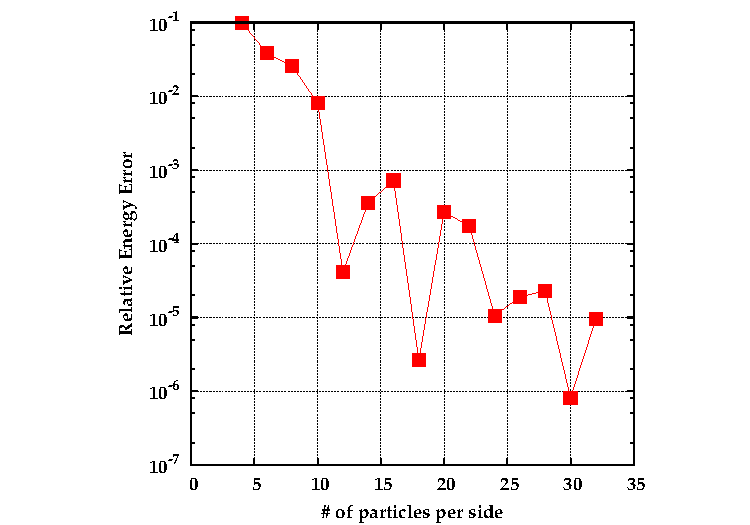
\includegraphics[width=10cm]{fig/p3m.pdf}
\caption{1辺あたりの粒子数とエネルギー相対誤差の関係(メッシュ数は$16^{3}$、カットオフ半径は$3/16$)}
\label{fig:p3m}
\end{figure}
\clearpage

\ifCpp % for C++
%=========================
%   TreePM コードの解説
%=========================
\subsection{TreePMコード} \label{subsec:TreePM}
本節では、FDPSの拡張機能 Particle Mesh (以下、PMと省略する)の使用方法について、TreePM(Tree-Particle-Mesh)法のサンプルコードを用いて解説を行う。このサンプルコードでは、宇宙論的$N$体シミュレーションをTreePM法を用いて実行する。TreePM法は第\ref{subsec:P3M}節で説明した$\mathrm{P^{3}M}$法と同様、重力計算をPPパートとPMパートにsplitして行う。したがって、使用するFDPSの機能は$\mathrm{P^{3}M}$法のサンプルコードとほぼ同じである。2つの方法の違いは、TreePM法ではPPパートの計算を直接法(ダイレクトサム法)ではなくTree法を使って計算する点にある。

\subsubsection{サンプルコードの場所と作業ディレクトリ}
サンプルコードの場所は、\path{$(FDPS)/sample/c++/treepm} である。まずは、そこに移動する。
下に示すように、サンプルコードは複数のファイルから構成される。
この内、FDPSに関係した部分は主に\texttt{treepm.hpp}と\texttt{treepm.cpp}に実装されている。
以下の説明では、適宜、ファイル名を参照していく。
\begin{screen}
\begin{verbatim}
$ cd (FDPS)/sample/c++/treepm
$ ls | awk '{print $0}'
IC/
Makefile
README_en.txt
README_ja.txt
constants.hpp
cosmology.hpp
fig/
make_directory.c
param_file_for_test.txt
prototype.h
result/
run_param.hpp
test.py*
timing.c
treepm.cpp
treepm.hpp
utils/
\end{verbatim}
\end{screen}

\subsubsection{ヘッダファイルのインクルード}
FDPSの標準機能と拡張機能の両方を使うため、メイン関数が定義されたファイル\texttt{treepm.cpp}で、\texttt{particle\_simulator.hpp}と\texttt{particle\_mesh.hpp}をインクルードしている:
\begin{lstlisting}[caption=Include FDPS]
#include <particle_simulator.hpp>
#include <particle_mesh.hpp>
\end{lstlisting}

\subsubsection{ユーザー定義クラス}
FDPSを使用するため、ユーザはユーザ定義クラスを実装しなければならない。
本節では、ユーザ定義クラスをサンプルコードでどのように実装しているかを説明する。

% FullParticle型
\subsubsubsection{FullParticle型}
ユーザーはFullParticle型を記述しなければならない。FullParticle型には、計算を行うにあたり、粒子が持っているべき全ての物理量が含まれている必要がある。Listing \ref{treepm_FP}に、サンプルコードのFullParticle型を示す。このサンプルコードでは通常の$N$体計算に必要なメンバ変数(\texttt{id}, \texttt{mass}, \texttt{eps}, \texttt{pos}, \texttt{vel}, \texttt{acc})に加え、PMパートの加速度を格納する\texttt{acc\_pm}、ハッブル定数を格納する\texttt{H0}、計算領域の大きさを$\mathrm{Mpc\;h^{-1}}$単位で格納する\texttt{Lbnd}が用意されている。また、FDPSの標準機能・拡張機能を使うため、以下のメンバ関数を持たせる必要がある:
\begin{itemize}[leftmargin=*,itemsep=-1ex]
\item \texttt{getCharge()} --- FDPSが粒子の質量を取得するのに必要
\item \texttt{getChargeParticleMesh()} --- FDPSのPMモジュールが粒子の電荷量を取得するために必要
\item \texttt{getPos()} --- FDPSが粒子座標を取得するのに必要
\item \texttt{getRSearch()} --- FDPSがカットオフ半径を取得するのに必要
\item \texttt{setPos()} --- FDPSが粒子の座標を書き込むのに必要
\item \texttt{copyFromForce()} --- Force型から結果をコピーするのに必要なメンバ関数
\item \texttt{copyFromForceParticleMesh()} --- PMモジュールが力の計算結果を書き込むために必要
\end{itemize}
さらに、FDPSの入出力関数を使用するため、以下のメンバ関数を定義してある:
\begin{itemize}[leftmargin=*,itemsep=-1ex]
\item \texttt{readBinary()}
\item \texttt{writeBinary()}
\end{itemize}
但し、この2つは必須ではなく、ユーザ独自の入出力関数を定義してもよい。

\lstinputlisting[linerange={31-222},caption=FullParticle型,label=treepm_FP]{../../../../sample/c++/treepm/treepm.hpp}

% EssentialParticleI型
\subsubsubsection{EssentialParticleI型}
ユーザーはEssentialParticleI型を記述しなければならない。EssentialParticleI型には、PPパートのForce計算を行う際、$i$粒子が持っているべき全ての物理量をメンバ変数として持っている必要がある。Listing \ref{treepm_EPI}に、サンプルコードのEssentialParticleI型を示す。このEssentialParticleI型には、前述したFullParticle型から値をコピーするのに必要なメンバ関数\texttt{copyFromFP()}と、EssentialParticleI型の粒子座標を返すメンバ関数\texttt{getPos()}を持たせる必要がある。

\lstinputlisting[linerange={231-247},caption=EssentialParticleI型,label=treepm_EPI]{../../../../sample/c++/treepm/treepm.hpp}

% EssentialParticleJ型
\subsubsubsection{EssentialParticleJ型}
ユーザーはEssentialParticleJ型を記述しなければならない。\ref{subsec:P3M}節の$\mathrm{P^{3}M}$コードの例では、EssentialParticleJ型はEssentialParticleI型で兼ねていたが、このサンプルコードでは別のクラスとして定義してある。EssentialParticleJ型には、PPパートのForce計算を行う際、$j$粒子が持っているべき全ての物理量をメンバ変数として持っている必要がある。Listing \ref{treepm_EPJ}に、サンプルコードのEssentialParticleJ型を示す。このEssentialParticleJ型には、以下のメンバ関数を持たせる必要がある:
\begin{itemize}[leftmargin=*,itemsep=-1ex]
\item \texttt{getPos()} --- FDPSが粒子位置を取得するのに必要
\item \texttt{getCharge()} --- FDPSが粒子質量を取得するのに必要
\item \texttt{copyFromFP()} --- FDPSがFullParticle型からEssentialParticleJ型に必要な情報を渡すのに必要
\item \texttt{getRSearch()} --- FDPSがカットオフ半径を取得するのに必要
\item \texttt{setPos()} --- FDPSが粒子座標を書き込むのに必要
\end{itemize}

\lstinputlisting[linerange={249-278},caption=EssentialParticleJ型,label=treepm_EPJ]{../../../../sample/c++/treepm/treepm.hpp}

% Force型
\subsubsubsection{Force型}
ユーザーはForce型を記述しなければならない。Force型は、PPパートのForceの計算を行った際にその結果として得られる全ての物理量をメンバ変数として持っている必要がある。本サンプルコードのForce型をListing \ref{treepm_force}に示す。Force型には積算対象のメンバ変数を0ないし初期値に設定するための関数\texttt{clear()}が必要になる。

\lstinputlisting[linerange={19-28},caption=Force型,label=treepm_force]{../../../../sample/c++/treepm/treepm.hpp}

% calcForceEpEp型
\subsubsubsection{calcForceEpEp型}
ユーザーはcalcForceEpEp型を記述しなければならない。calcForceEpEp型には、PPパートのForceの計算の具体的な内容を書く必要がある。サンプルコードのcalcForceEpEp型をListing \ref{treepm_calcForceEpEp}に示す。このサンプルコードでは、calcForceEpEp型はファンクタ(関数オブジェクト)として実装されている(テンプレート関数として実装されていることに注意されたい)。また、Phantom-GRAPEライブラリを使用するかどうかに応じて(マクロ定義\texttt{ENABLE\_PHANTOM\_GRAPE\_X86}で判定している)、場合分けして実装されている。いずれの場合でも、ファンクタの引数は、EssentialParticleIの配列、EssentialParticleIの個数、EssentialParticleJの配列、EssentialParticleJの個数、Force型の配列である。

\lstinputlisting[linerange={344-365},caption=calcForceEpEp型,label=treepm_calcForceEpEp]{../../../../sample/c++/treepm/treepm.hpp}

TreePM法のPPパートは、$\mathrm{P^{3}M}$法と同様、距離に関するカットオフ付きの2体相互作用である。そのため、ここでも加速度計算にカットオフ関数が掛かる。\ref{subsubsubsec:p3m_calcForceEpEp}節で解説したように、カットオフ関数はHockney \& Eastwood (1988)の$S2$型の粒子形状関数に対応したカットオフ関数である必要がある。Phantom-GRAPEライブラリを使用しない場合の実装では、カットオフ関数が関数\texttt{gfactor\_S2()}として定義されている。一方、Phantom-GRAPEライブラリを使用する場合には、カットオフが考慮されたバージョンのPhantom-GRAPEライブラリが使用されるようになっている。Phantom-GRAPEライブラリに指定したカットオフ半径で計算させるため、API \texttt{pg5\_gen\_s2\_force\_table()}を事前に呼び出しておく必要がある。サンプルコードでは、メイン関数でこれを行っている:
\begin{lstlisting}
#ifdef ENABLE_PHANTOM_GRAPE_X86 
    //g5_open();
    pg5_gen_s2_force_table(EPS_FOR_PP, 3.0/SIZE_OF_MESH);
#endif
\end{lstlisting}

% プログラム本体
\subsubsection{プログラム本体}
本節では、サンプルコード本体について解説を行う。詳細な説明に入る前に、サンプルコー ドの内容と全体構造について説明を与える。\ref{subsec:TreePM}節冒頭で述べたように、このサンプルコードでは宇宙論的$N$体シミュレーションをTreePM法を用いて実行する。初期条件としては、以下の3つの場合に対応している:
\begin{enumerate}[leftmargin=*,itemsep=-1ex,label=(\alph*)]
\item Santa Barbara Cluster Comparison Test
  (\href{http://iopscience.iop.org/article/10.1086/307908/meta}{Frenk
  et al.[1999, ApJ, 525, 554]})で用いられた初期条件(\url{https://v2.jmlab.jp/owncloud/index.php/s/XnzvW5XAYwfqZYQ?path=%2Fsb}から初期条件を入手可能。ファイル \path{ic_sb128.tar} は粒子数$128^3$のデータ、ファイル \path{ic_sb256.tar} は粒子数$256^3$のデータ)
\item 上記テストで用いられた初期条件ファイルと同じフォーマットで記述された初期条件
\item ランダムにおいた粒子分布
\end{enumerate}
実行時のコマンドライン引数として初期条件を指定した後、初期条件ファイル内で指定された終了時刻(赤方偏移$z$)まで、TreePM法で粒子の運動を計算する。各初期条件に対応したパラメータファイルのファイルフォーマットについては、\path{$(FDPS)/sample/c++/treepm/README_ja.txt} で説明されているので、そちらを参照されたい。また、\path{$(FDPS)/sample/c++/treepm/result/input.para} に、(a)の場合のパラメータファイルの記述例があるので、そちらも参照されたい。

コード全体の構造は以下のようになっている:
\begin{enumerate}[leftmargin=*,itemsep=-1ex,label=(\arabic*)]
\item FDPSで使用するオブジェクトの生成と初期化
\item (必要であれば)Phantom-GRAPEライブラリの初期化
\item 初期条件ファイルの読み込み
\item 終了時刻まで粒子の運動を計算
\end{enumerate}

以下で、個々について詳しく説明を行う。

\subsubsubsection{開始、終了}
まずは、FDPSの初期化/開始を行う必要がある。
次のように、メイン関数に記述する。
\begin{lstlisting}[caption=FDPSの開始]
PS::Initialize(argc, argv);
\end{lstlisting}

FDPSは、開始したら明示的に終了させる必要がある。
今回は、プログラムの終了と同時にFDPSも終了させるため、メイン関数の最後に次のように記述する。
\begin{lstlisting}[caption=FDPSの終了]
PS::Finalize();
\end{lstlisting}

\subsubsubsection{オブジェクトの生成と初期化}
FDPSの初期化に成功した場合、ユーザーはコード中で用いるオブジェクトを作成する必要がある。
本節では、オブジェクトの生成/初期化の仕方について、解説する。

\subsubsubsubsection{オブジェクトの生成}
TreePM法の計算では、$\mathrm{P^{3}M}$法のときと同様、粒子群クラス、領域クラス、PPパートの計算で使用するtreeを1本、そして、PMパートの計算に必要なParticleMeshオブジェクトの生成が必要である。本サンプルコードでは、\texttt{treepm.cpp}のメイン関数内でオブジェクトの生成が行われている:
\begin{lstlisting}[caption=オブジェクトの生成]
int main(int argc, char **argv)
{
   PS::PM::ParticleMesh pm;
   PS::ParticleSystem<FPtreepm> ptcl;
   PS::DomainInfo domain_info;
   PS::TreeForForceLong<Result_treepm, EPItreepm, EPJtreepm>::MonopoleWithCutoff treepm_tree;
}
\end{lstlisting}
上記はサンプルコードからオブジェクト生成部分だけを抜き出してきたものであることに注意されたい。

\subsubsubsubsection{オブジェクトの初期化}
ほとんどのFDPSのオブジェクトは、生成後、初期化してから使用する必要がある。前節で説明した4つのオブジェクトの内、明示的な初期化が不要なのはParticleMeshクラスである。それ以外のオブジェクトに関しては、\texttt{initialize}メソッドで初期化を行う。以下に、サンプルコードでのオブジェクトの初期化を示す:
\begin{lstlisting}[caption=オブジェクトの初期化]
int main(int argc, char **argv)
{
   // Initialize ParticleSystem
   ptcl.initialize();

   // Initialize DomainInfo
   domain_info.initialize();  
   domain_info.setBoundaryCondition(PS::BOUNDARY_CONDITION_PERIODIC_XYZ);
   domain_info.setPosRootDomain(PS::F64vec(0.0, 0.0, 0.0), 
                                PS::F64vec(1.0, 1.0, 1.0));
                                
   // Initialize Tree
   treepm_tree.initialize(3*ptcl.getNumberOfParticleGlobal(),
                          this_run.theta);
}
\end{lstlisting}

粒子群クラスのオブジェクトの初期化は、単に\texttt{initialize}メソッドを引数無しで呼び出すだけである。


領域クラスに関しては、\texttt{initialize}メソッド呼び出し後に、境界条件と境界の大きさを指定する必要がある。
これらはそれぞれ\texttt{setBoundaryCondition}メソッドと\texttt{setPosRootDomain}メソッドで行う。

ツリーオブジェクトの初期化の際には、\texttt{initialize}メソッドに計算で使用する大雑把な粒子数を第1引数として渡す必要がある。本サンプルコードでは、全粒子数の3倍の値を渡している。第2引数には、tree法で力の計算を行う際のopening angle criterion $\theta$を指定する。本サンプルコードでは、$\theta$をはじめとした、計算を制御するパラメータ群を構造体\texttt{this\_run}のメンバ変数としてまとめている。


\subsubsubsection{初期条件の設定}
初期条件を指定するパラメータファイルの読み込みは、メイン関数で呼ばれる関数\texttt{read\_param\_file()}内で行われる:
\begin{lstlisting}
read_param_file(ptcl, this_run, argv[1]);
\end{lstlisting}
この関数ではプログラム実行時に指定されたパラメータファイルを読み込み、粒子群クラスのオブジェクト\texttt{ptcl}に粒子データをセットする。サンプルコードでは、この後、FDPSのAPIを使って、領域分割と粒子交換を行っている。以下でこれらのAPIについて解説する。

\subsubsubsubsection{領域分割の実行}
粒子分布に基いて領域分割を実行するには、領域クラスの\texttt{decomposeDomainAll}メソッドを使用する:
\begin{lstlisting}[caption=領域分割の実行]
domain_info.decomposeDomainAll(ptcl);
\end{lstlisting}
ここで、粒子分布の情報を領域クラスに与えるため、引数に粒子群クラスのオブジェクトが渡されていることに注意されたい。
この領域分割はメイン関数内で行われている。


\subsubsubsubsection{粒子交換の実行}
領域情報に基いてプロセス間の粒子の情報を交換するには、粒子群クラスの\texttt{exchangeParticle}メソッドを使用する:
\begin{lstlisting}[caption=粒子交換の実行]
ptcl.exchangeParticle(domain_info);
\end{lstlisting}
ここで領域情報を粒子群クラスに与えるため、引数に領域クラスのオブジェクトが渡されていることに注意する。

\subsubsubsection{相互作用計算の実行}
領域分割・粒子交換が完了したら、計算開始時の加速度を決定するため、相互作用計算を行う必要がある。
以下に、本サンプルコードでの相互作用計算の実装を示す。
本サンプルコードでは、PPパートの計算にはツリーオブジェクトの\texttt{calcForceAllAndWriteBack}メソッドを使用している。
このメソッドを実行することで、粒子群オブジェクトのメンバ変数\texttt{acc}にPPパートの加速度が格納される。
PMパートの計算にはParticleMeshオブジェクトの\texttt{calcForceAllAndWriteBack}メソッドを使用している。
これによって、粒子群クラスのメンバ変数\texttt{acc\_pm}にPMパートの加速度が格納される。

\begin{lstlisting}[caption=相互作業計算の実行]
//* PP part
treepm_tree.calcForceAllAndWriteBack
    (calc_pp_force<EPJtreepm>(),
     calc_pp_force<PS::SPJMonopoleCutoff>(),
     ptcl,
     domain_info);
 
//* PM part
pm.calcForceAllAndWriteBack(ptcl, domain_info); 
\end{lstlisting}

\subsubsubsection{時間積分ループ}
本サンプルコードでは、時間積分をLeapfrog時間積分法によって行っている(この方法に関しては、\ref{s4sec:nbody_time_integration}節を参照されたい)。粒子位置を時間推進する$D(\cdot)$オペレータは関数\texttt{drift\_ptcl}、粒子速度を時間推進する$K(\cdot)$オペレータは関数\texttt{kick\_ptcl}として実装されている。宇宙膨張の効果は関数\texttt{kick\_ptcl}内で考慮されている。また、スケールファクターやハッブルパラメータの時間発展は構造体\texttt{this\_run}のメンバ関数\texttt{update\_expansion}で計算されている。

\subsubsection{コンパイル}
README.txtで説明されているように、Makefileを適宜編集し、\texttt{make}コマンドを実行することでコンパイルすることができる。$\mathrm{P^{3}M}$コード同様、本サンプルコードでもFFTWライブラリを使用するため、ユーザ自身でインストールする必要がある。コンパイルが成功すれば、実行ファイル\texttt{treepm}が作成されているはずである。

\subsubsection{実行}
FDPSの拡張機能ParticleMeshの仕様上、プロセス数が2以上のMPI実行でなければ正常に動作しない。
そこで、以下のように実行する必要がある:
\begin{screen}
\begin{verbatim}
$ MPIRUN -np NPROC ./treepm
\end{verbatim}
\end{screen}
ここで、"MPIRUN"にはmpirunやmpiexecなどのMPI実行プログラムが、"NPROC"にはプロセス数が入る。

\subsubsection{結果の確認}
計算が終了するとパラメータファイルで指定されたディレクトリに計算結果が出力されるはずである。
粒子数$256^{3}$で、Santa Barbara Cluster Comparison Testを実行した場合の、ダークマター密度分布の時間発展の様子を図\ref{fig:treepm}に示す。

\begin{figure}[h]
\centering
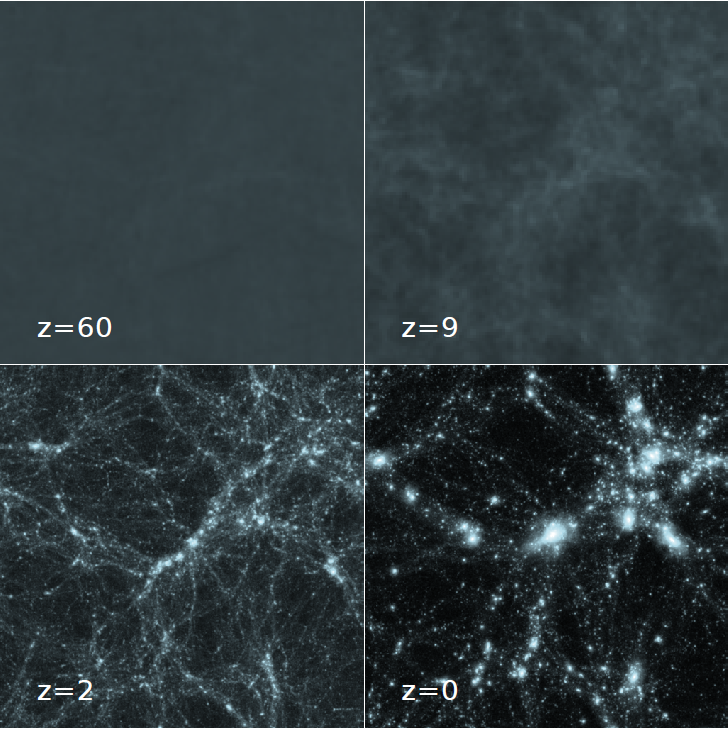
\includegraphics[width=0.666\linewidth]{./fig/sb256.png}
\caption{Santa Barbara Cluster Comparison テストの密度分布の時間発展(粒子数$256^{3}$)}
\label{fig:treepm}
\end{figure}

\endifCpp % \ifCpp はTreePMコードの節全体に掛かっている.